\chapter{Tervezés}

Ez a fejezet az alkalmazás tervezési döntéseit mutatja be: az architektúrától az adatmodellen és a biztonsági megfontolásokon át a felhasználói felület logikájáig. A tervezési szakasz célja, hogy a megvalósítás előtt strukturált, konzisztens alapot fektessen le, csökkentve a fejlesztés közbeni átdolgozások szükségességét.

% ============================================================
%  3.1  Rendszerarchitektúra
% ============================================================
\section{Rendszerarchitektúra}

\subsection{Háromrétegű architektúra}

Az alkalmazás klasszikus háromrétegű (three-tier) architektúrát követ, amelyet a Spring MVC keretrendszer természetes módon kényszerít ki:

\begin{itemize}
    \item \textbf{Megjelenítési réteg (Presentation Layer):} Thymeleaf HTML sablonok, CSS stíluslapok és a böngésző oldali megjelenítés. Ez a réteg felelős a felhasználói interakciók fogadásáért és az adatok vizuális megjelenítéséért.
    \item \textbf{Üzleti logika réteg (Business Layer):} Spring MVC kontrollerek és service osztályok. A kontrollerek a HTTP kérések fogadásáért és az eredmények visszaküldéséért felelnek, míg a service osztályok az alkalmazás üzleti szabályait valósítják meg.
    \item \textbf{Adatelérési réteg (Data Access Layer):} Spring Data JPA repository interfészek és a H2 adatbázis. Ez a réteg absztrahálja az adatbázis-műveleteket, lehetővé téve, hogy az üzleti logika réteg ne függjön közvetlenül az adatbázis típusától.
\end{itemize}

A rétegek közötti kommunikáció szigorúan egyirányú: a kontroller hívja a service-t, a service hívja a repository-t, a repository pedig az adatbázissal kommunikál. Ez a felépítés megfelel a \textit{Separation of Concerns} elvének, és megkönnyíti az egyes rétegek önálló tesztelhetőségét, cserélhetőségét.

\subsection{Kérés-feldolgozás folyamata}

Egy tipikus HTTP kérés feldolgozása az alábbi lépéseken megy keresztül:

\begin{enumerate}
    \item A böngésző HTTP kérést küld a szervernek (pl. \texttt{GET /courses}).
    \item A Spring Security \texttt{SecurityFilterChain} ellenőrzi, hogy a kérés hitelesített-e, és a felhasználó rendelkezik-e a szükséges jogosultsággal.
    \item A \texttt{DispatcherServlet} az URL és a HTTP metódus alapján meghatározza a megfelelő kontrollert és metódust.
    \item A kontroller meghívja a szükséges service metódusokat az üzleti logika végrehajtásához.
    \item A service a repository interfészeken keresztül lekéri vagy módosítja az adatbázisban tárolt adatokat.
    \item A kontroller az eredményt egy \texttt{Model} objektumba helyezi, és visszaadja a nézet nevét.
    \item A Thymeleaf sablon-motor a modell adatai alapján legenerálja a HTML választ.
    \item A böngésző megjeleníti a visszakapott HTML oldalt.
\end{enumerate}

\subsection{Telepítési modell}

Az alkalmazás egyetlen önálló JAR-fájlként terjeszthető, amely magában foglalja a beágyazott Tomcat alkalmazásszervert. Ez lényegesen egyszerűsíti a telepítést: nincs szükség különálló alkalmazászerverr konfigurálására. A fejlesztési fázisban beágyazott H2 memória-adatbázis kerül alkalmazásra, amelyet éles környezetben PostgreSQL vagy MySQL adatbázisra lehet felváltani mindössze az \texttt{application.properties} módosításával, a Java forráskód megváltoztatása nélkül. Ez a rugalmasság a Spring Data JPA adatbázis-agnosztikus absztrakciójából következik.

% ============================================================
%  3.2  Adatmodell
% ============================================================
\section{Adatmodell}

Az alkalmazás adatmodellje nyolc entitást tartalmaz, amelyek JPA annotációkkal vannak leképezve relációs táblákra. Az entitások tervezésekor a normalizált adatszerkezet és az egyszerű lekérdezhetőség szempontjai egyaránt érvényesültek.

\newpage

\begin{figure}[h!]
    \centering
    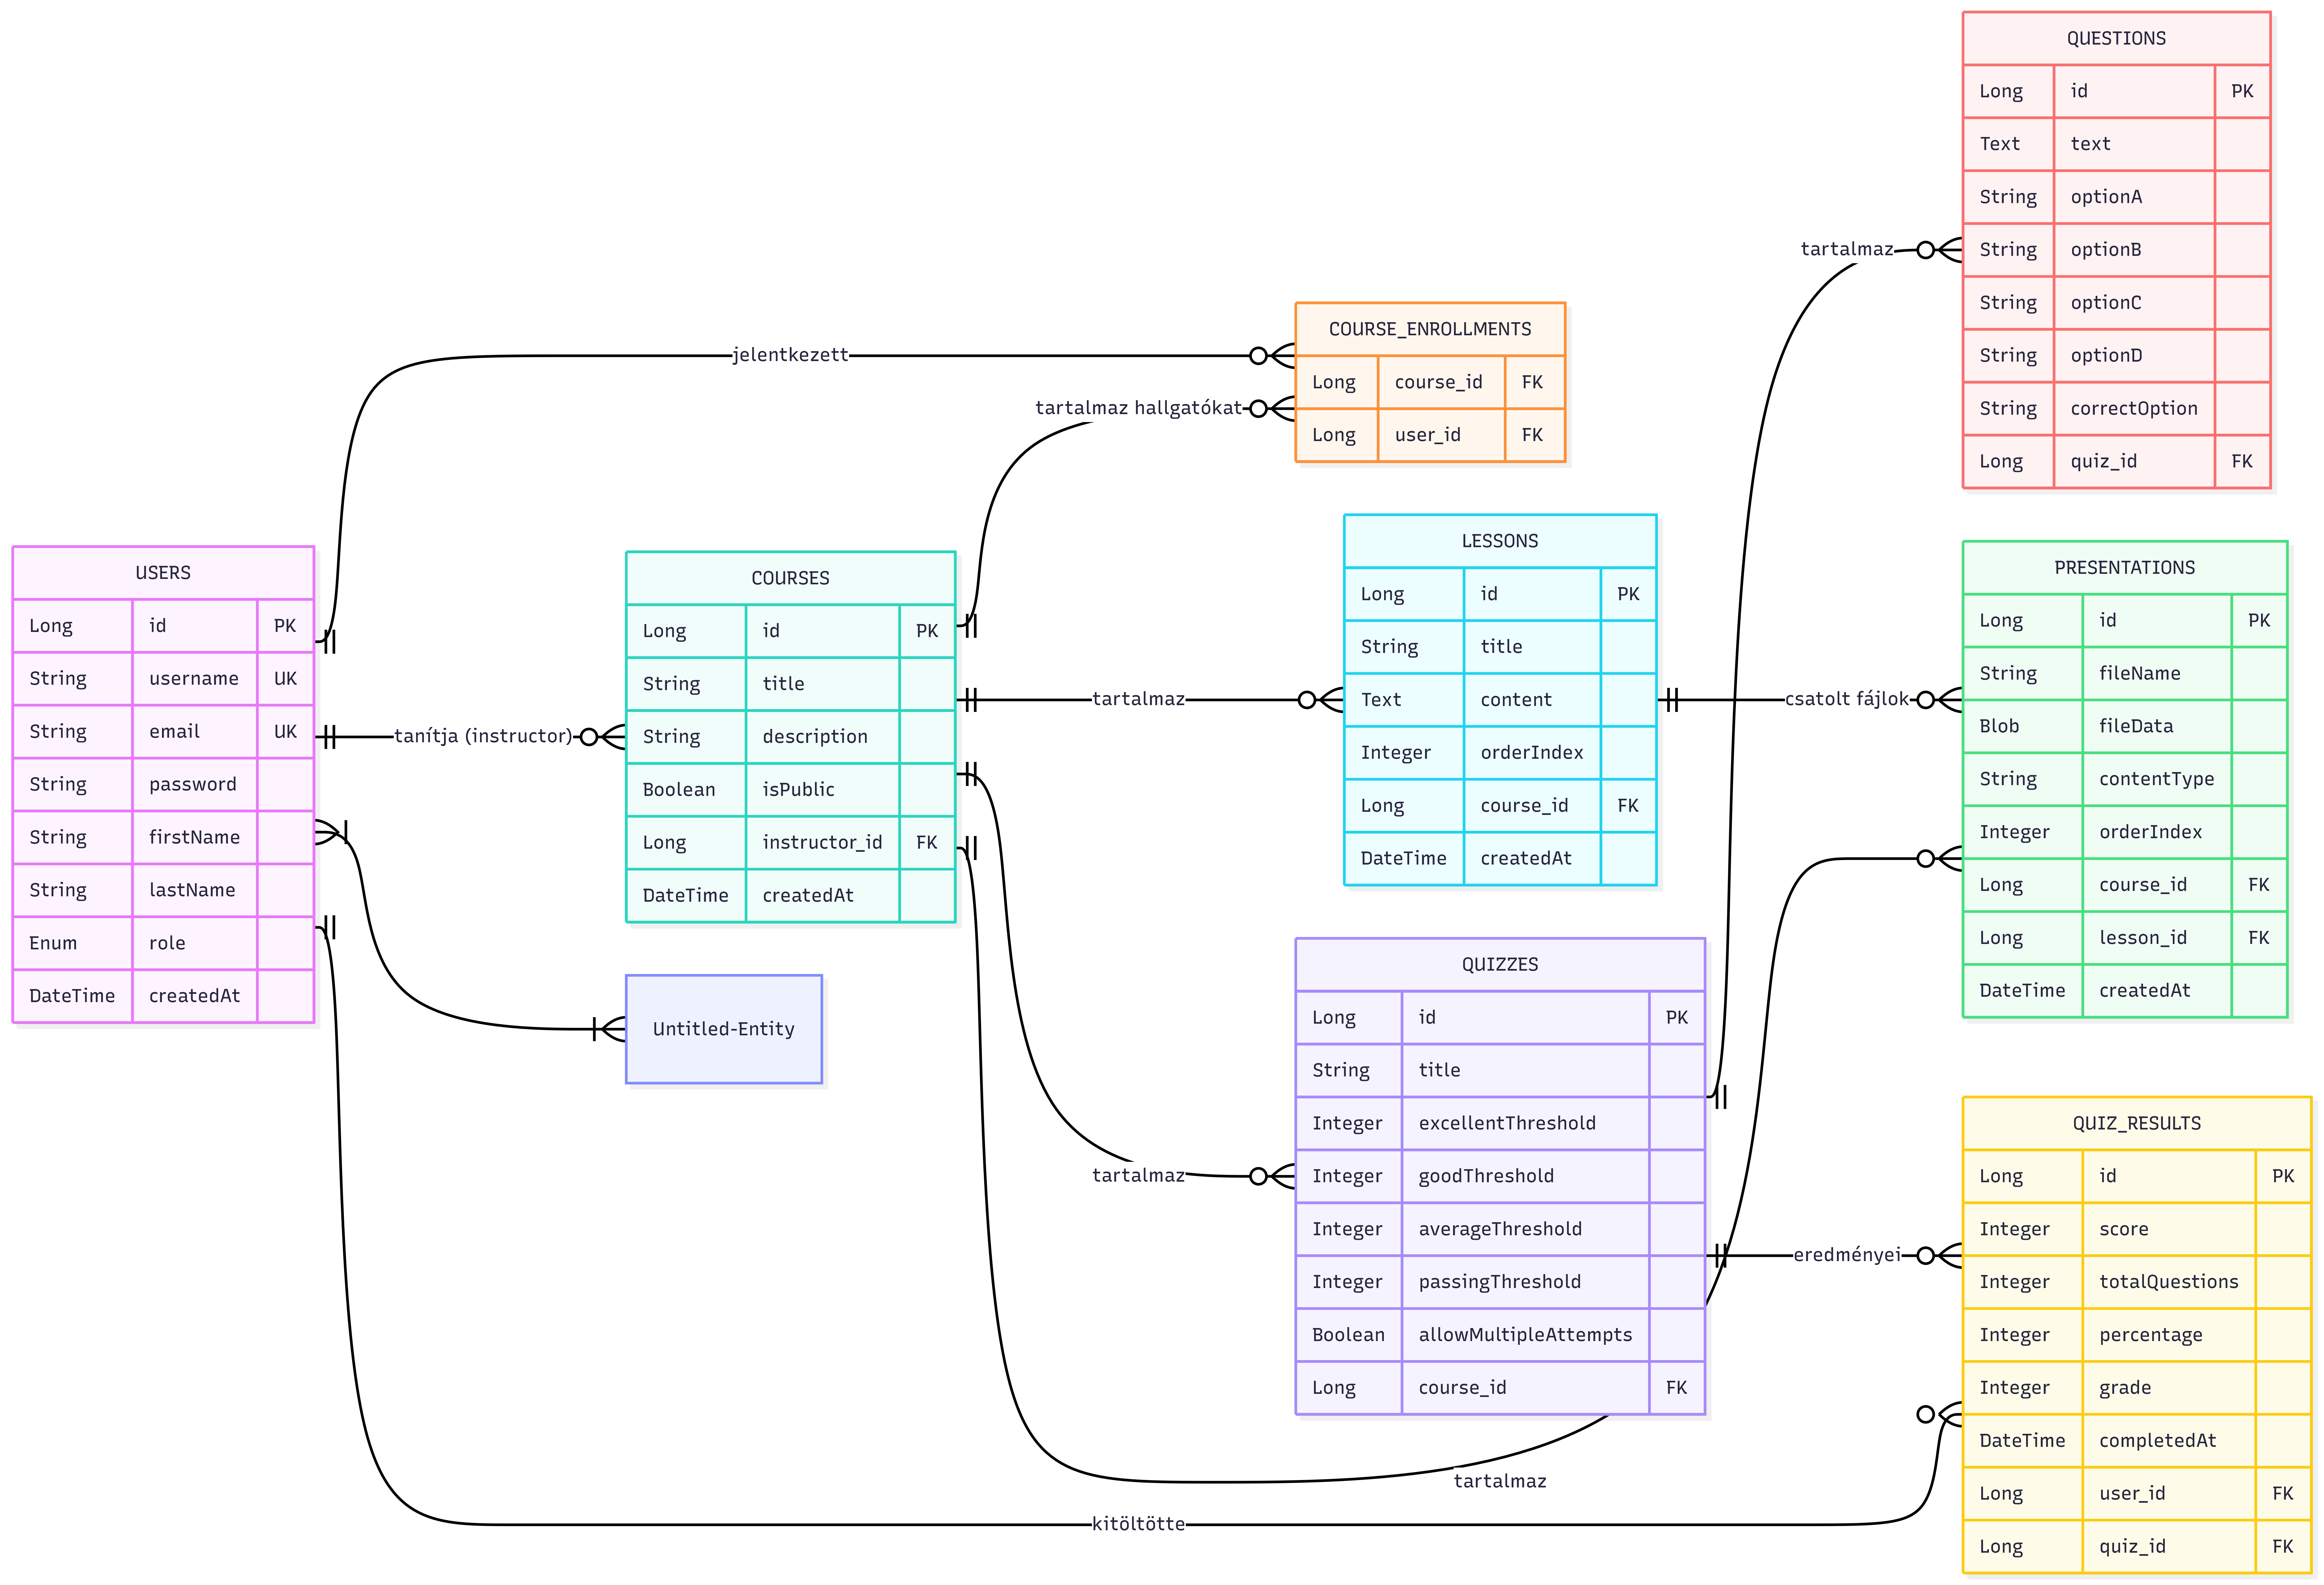
\includegraphics[width=1\textwidth]{images/Adatbazis_sema.png}
    \caption{Az adatbázis logikai sémája}
    \label{fig:Adatbazis_sema}
\end{figure}

\subsection{User}

A \texttt{User} entitás tárolja a felhasználói adatokat: egyedi felhasználónév (\texttt{username}), e-mail cím (\texttt{email}), titkosított jelszó (\texttt{password}), keresztnév (\texttt{firstName}), vezetéknév (\texttt{lastName}), szerepkör (\texttt{role}: \texttt{ADMIN}, \texttt{INSTRUCTOR} vagy \texttt{STUDENT}) és a regisztráció dátuma (\texttt{createdAt}). Egy felhasználó több kurzusra is beiratkozhat, amelyet \texttt{@ManyToMany} kapcsolat valósít meg a \texttt{Course} entitással, egy köztes \texttt{user\_courses} kapcsolótáblán keresztül.

A tervezés során tudatos döntés volt, hogy a szerepkör nem külön táblában, hanem egyetlen enum mezőben tárolódik. Ez az egyszerűsítés az alkalmazás léptékéhez igazodik: három, előre rögzített szerepkörrel egy JOIN-műveletet megtakarít minden lekérdezésnél, anélkül hogy a kibővíthetőséget lényegesen korlátozná.

\subsection{Course}

A \texttt{Course} entitás képviseli a kurzusokat. Tartalmaz címet (\texttt{title}), leírást (\texttt{description}), nyilvánossági jelzőt (\texttt{isPublic}), az oktató referenciáját (\texttt{instructor}, \texttt{@ManyToOne} kapcsolat a \texttt{User} entitással), leckék listáját (\texttt{lessons}, \texttt{@OneToMany}), kvízek listáját (\texttt{quizzes}, \texttt{@OneToMany}), prezentációk listáját (\texttt{presentations}, \texttt{@OneToMany}), valamint a beiratkozott hallgatók halmazát (\texttt{enrolledStudents}, \texttt{@ManyToMany}).

Az \texttt{isPublic} jelző lehetővé teszi, hogy egyes kurzusok szabadon böngészhetők és csatlakozhatók legyenek, míg más kurzusokba csak az oktató explicit engedélyével lehet belépni. Ez a kétszintű láthatósági modell rugalmasságot biztosít az oktatóknak.

\subsection{Lesson}

A \texttt{Lesson} egy kurzuson belüli tematikus leckét jelöl. Tartalmaz egy sorszámot (\texttt{orderIndex}), amely meghatározza a leckék megjelenítési sorrendjét a kurzuson belül, szöveges tartalmat (\texttt{content}, adatbázisban \texttt{TEXT} típusú oszlopban tárolva), a lecke létrehozásának időpontját (\texttt{createdAt}), valamint hivatkozást a szülő kurzusra (\texttt{course}, \texttt{@ManyToOne} kapcsolat a \texttt{Course} entitással). Emellett a lecke közvetlen kapcsolatban áll a hozzá feltöltött prezentációkkal is (\texttt{presentations}, \texttt{@OneToMany} kapcsolat a \texttt{Presentation} entitással, \texttt{CascadeType.ALL} beállítással).
Ez utóbbi kapcsolat teszi lehetővé a lecke-szintű anyagszervezést: az oktató a prezentációkat nem csupán kurzusszinten, hanem konkrét leckékhez rendelve is feltöltheti, így a hallgatók a kurzus megtekintésekor tematikusan, leckénként is böngészhetnek a feltöltött anyagok között. A \texttt{Presentation} entitás \texttt{lesson} mezője opcionális (lehet \texttt{null}), ami azt jelenti, hogy a korábbi, leckéhez nem rendelt kurzusszintű prezentációk is érvényes állapotban maradnak.
A sorrend külön mezőben való tárolása lehetővé teszi, hogy az oktatók tetszőlegesen rendezhessék a leckéket az adatbázis-sorok fizikai sorrendjének megváltoztatása nélkül. A leckék lekérdezése mindig az \texttt{orderIndex} mező szerint növekvő sorrendben történik.

\subsection{Presentation}

A \texttt{Presentation} a feltöltött prezentációs anyagot reprezentálja. Tárolja az eredeti fájlnevet (\texttt{originalFilename}), a fájl bináris adatait \texttt{byte[]} tömbként (\texttt{fileData}), a fájl MIME-típusát (\texttt{contentType}), valamint a szülő kurzus referenciáját (\texttt{course}, \texttt{@ManyToOne}). A bináris tartalom adatbázisban való tárolása egyszerűsíti a telepítést, hiszen nincs szükség külön fájlrendszer-kezelésre; ugyanakkor éles, nagy forgalmú környezetben ez a megközelítés felváltható objektumtárolóval (pl. Amazon S3).

\subsection{Quiz és Question}

A \texttt{Quiz} egy kurzushoz rendelt tesztet jelöl (\texttt{@ManyToOne} kapcsolat a \texttt{Course}-szal). Tartalmazza a kvíz nevét (\texttt{title}), azt, hogy engedélyezett-e többszöri kitöltés (\texttt{allow\-Multiple\-Attempts}), a ponthatárokat (pl. \texttt{thresholdExcellent}, \texttt{thresholdGood} stb.), valamint a kérdések listáját (\texttt{questions}, \texttt{@OneToMany}).

A \texttt{Question} entitás egyedi kérdést tárol (\texttt{questionText}), a lehetséges válaszlehetőségeket (\texttt{options}, \texttt{List<String>}, amelyet JPA \texttt{@ElementCollection} segítségével külön táblában tárol), és a helyes válasz nullaalapú indexét (\texttt{correctAnswerIndex}). Az \texttt{@ElementCollection} használatával a válaszlehetőségek száma kérdésenként rugalmasan változhat, ami az adatmodell módosítása nélkül is jelentősen megkönnyíti a jövőbeli, eltérő struktúrájú kérdéstípusok implementálását.

\begin{figure}[h!]
    \centering
    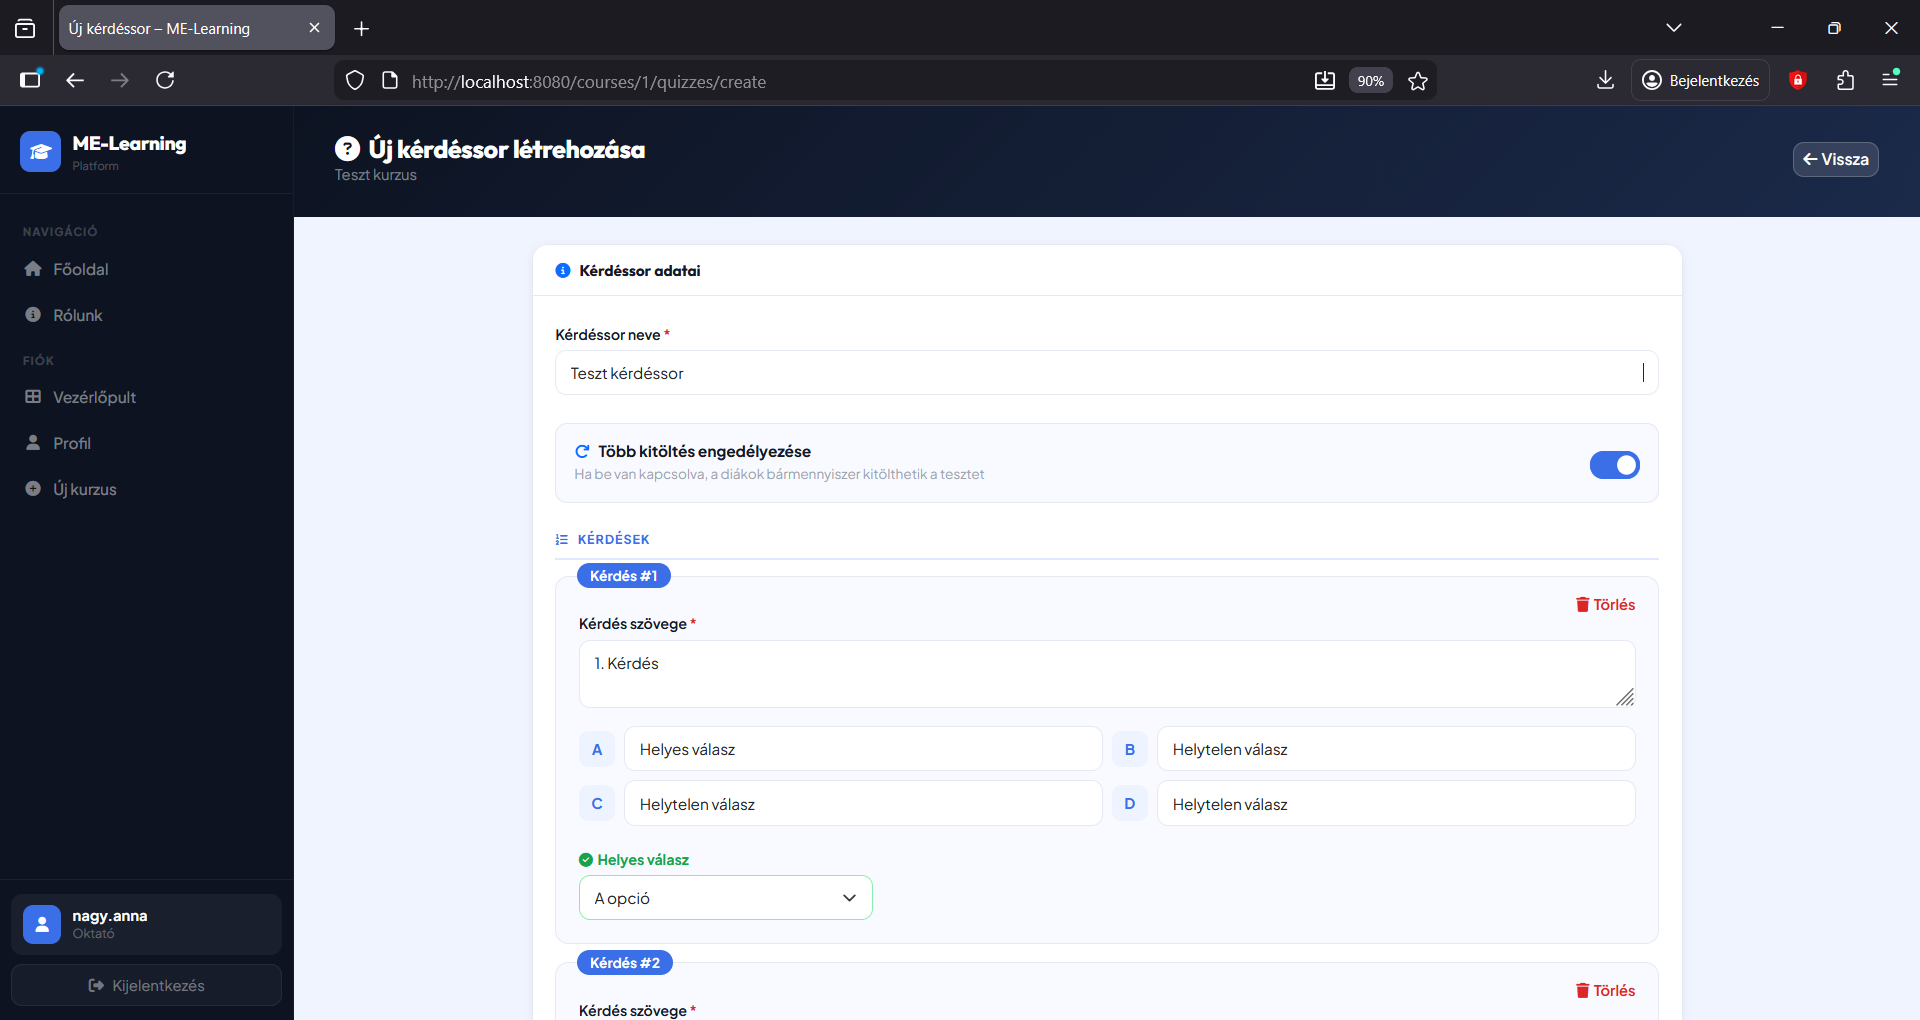
\includegraphics[width=1\textwidth]{images/Kerdessor_letrehozasa.png}
    \caption{Kérdéssor létrehozása}
    \label{fig:Kerdessor_letrehozasa}
\end{figure}

\subsection{QuizResult}

A \texttt{QuizResult} rögzíti egy hallgató kvízkitöltésének eredményét: hivatkozást a kitöltő felhasználóra (\texttt{user}, \texttt{@ManyToOne}), hivatkozást a kvízre (\texttt{quiz}, \texttt{@ManyToOne}), a szerzett pontszámot (\texttt{score}), a maximálisan elérhető pontszámot (\texttt{maxScore}), a kitöltés időpontját (\texttt{completedAt}) és a generált osztályzatot (\texttt{grade}). Az osztályzat a ponthatárok alapján kerül kiszámításra, és a kvíz ponthatárainak utólagos módosításakor automatikusan újraszámításra kerül.

\subsection{Role}

A \texttt{Role} egy Java \texttt{enum} típus, amely az \texttt{ADMIN}, \texttt{INSTRUCTOR} és \texttt{STUDENT} értékeket veheti fel. JPA szinten \texttt{@Enumerated(EnumType.STRING)} annotációval tárolódik, ami olvashatóbb adatbázis-tartalmat eredményez, és megvéd az enum-sorrend megváltozásából eredő hibáktól.

\subsection{Entitáskapcsolatok összefoglalása}

\begin{table}[h]
\centering
\caption{Az adatmodell entitásai és főbb kapcsolataik}
\label{tab:entities}
\begin{tabular}{|l|l|l|l|}
\hline
\textbf{Forrás entitás} & \textbf{Kapcsolat típusa} & \textbf{Cél entitás} & \textbf{Szemantika} \\
\hline
User & ManyToMany & Course & Hallgatói beiratkozás \\
Course & ManyToOne & User & Oktató tulajdonlás \\
Course & OneToMany & Lesson & Leckék listája \\
Course & OneToMany & Quiz & Kvízek listája \\
Course & OneToMany & Presentation & Feltöltött anyagok \\
Quiz & OneToMany & Question & Kérdések listája \\
QuizResult & ManyToOne & User & Kitöltő hallgató \\
QuizResult & ManyToOne & Quiz & Kitöltött kvíz \\
\hline
\end{tabular}
\end{table}

% ============================================================
%  3.3  Biztonsági tervezés
% ============================================================
\section{Biztonsági tervezés}

\subsection{Szerepkör-alapú hozzáférés-vezérlés}

Az alkalmazás szerepkör-alapú hozzáférés-vezérlést (Role-Based Access Control, RBAC) alkalmaz. A három szerepkör hierarchikusan épül egymásra:

\begin{itemize}
    \item \textbf{STUDENT:} A legszélesebb felhasználói csoport. Böngészhetik és megtekinthetik a nyilvános kurzusokat, beiratkozhatnak, megtekinthetik a feltöltött prezentációkat, és kitölthetik a kvízeket. Saját eredményeiket és profiljukat megtekinthetik.
    \item \textbf{INSTRUCTOR:} A STUDENT jogosultságain felül kurzusokat hozhatnak létre, szerkeszthetnek és törölhetnek, prezentációkat tölthetnek fel, kvízeket kezelhetnek, és kezelhetik a saját kurzusaikra beiratkozott hallgatókat. Más oktatók kurzusait nem módosíthatják.
    \item \textbf{ADMIN:} Teljes hozzáféréssel rendelkezik. Minden kurzust kezelhet a tulajdonostól függetlenül, a felhasználói fiókok tekintetében pedig törlési jogosultsággal bír.
\end{itemize}

\subsection{URL-szintű hozzáférés-vezérlés}

A Spring Security \texttt{SecurityFilterChain} konfiguráció URL-minta alapján szabályozza a hozzáférést. A tervezés során az alábbi hozzáférési zónákat határoztuk meg:

\begin{table}[h]
\centering
\caption{URL-zónák és hozzáférési szabályok}
\label{tab:security}
\begin{tabular}{|l|l|}
\hline
\textbf{URL-minta} & \textbf{Szükséges jogosultság} \\
\hline
\texttt{/}, \texttt{/login}, \texttt{/register}, \texttt{/about} & Nyilvános (hitelesítés nélkül) \\
\texttt{/courses}, \texttt{/courses/\{id\}/view} & Hitelesített felhasználó \\
\texttt{/courses/create}, \texttt{/courses/*/manage} & INSTRUCTOR vagy ADMIN \\
\texttt{/courses/*/quizzes/create} & INSTRUCTOR vagy ADMIN \\
Minden egyéb & Hitelesített felhasználó \\
\hline
\end{tabular}
\end{table}

Emellett a service rétegben is érvényesülnek tulajdonosi ellenőrzések: például a kurzus törlése előtt a rendszer ellenőrzi, hogy a bejelentkezett felhasználó a kurzus oktatója-e, vagy adminisztrátor-e. Ez a kétrétegű ellenőrzés védelmet nyújt a közvetlen URL-manipulációs kísérletek ellen is.

\subsection{Jelszókezelés}

A jelszavak tárolása BCrypt algoritmussal történik, amely egy adaptív, szándékosan lassú hash-függvény. A BCrypt automatikusan sózza (salt) a jelszavakat, így azonos jelszavak is különböző hash-értéket kapnak, ami megvéd a rainbow table alapú támadások ellen. A \texttt{BCryptPasswordEncoder} alapértelmezett erőssége (cost factor 10) iparági standardnek megfelelő védelmet biztosít.

\subsection{Munkamenet-kezelés}

A Spring Security alapértelmezett munkamenet-kezelését alkalmazzuk: a bejelentkezés után a felhasználó azonosítója HTTP munkamenetben (session cookie-ban) tárolódik. A munkamenet CSRF (Cross-Site Request Forgery) védelemmel egészül ki, amelyet a Spring Security automatikusan aktivál. Minden állapotváltoztató HTTP POST kérésnek tartalmaznia kell a szerver által generált CSRF tokent, amelyet a Thymeleaf sablonok \texttt{th:action} attribútuma automatikusan beilleszt.

% ============================================================
%  3.4  Felhasználói felület tervezése
% ============================================================
\section{Felhasználói felület tervezése}

\subsection{Általános UX-elvek}

A felhasználói felület tervezésekor a következő elvek érvényesültek:

\begin{itemize}
    \item \textbf{Szerepkör-tudatos megjelenítés:} A felhasználói felület dinamikusan alkalmazkodik a bejelentkezett felhasználó szerepköréhez. A Thymeleaf \texttt{sec:authorize} direktívája segítségével egyes elemek (pl. „Kurzus létrehozása" gomb, szerkesztési ikonok) csak az arra jogosult szerepkörök számára jelennek meg.
    \item \textbf{Visszajelzés és validáció:} Minden form esetén a szerver oldali validáció (Bean Validation / \texttt{@Valid}) azonnali visszajelzést ad a felhasználónak a hibás adatokról, és a korábban megadott helyes adatokat megőrzi az újratöltés után.
    \item \textbf{Konzisztens navigáció:} Minden autentikált oldal egységes fejléccel, navigációs sávval és oldalsávval rendelkezik, amelyet az újrafelhasználható \texttt{fragments/sidebar.html} Thymeleaf komponens valósít meg.
    \item \textbf{Reszponzív elrendezés:} A CSS stíluslapok mobilbarát elrendezést biztosítanak, amely különböző képernyőméreteken is használható marad.
\end{itemize}

\subsection{Oldalak és navigációs folyamatok}

Az alkalmazás nézetei három fő területre oszthatók:

\textbf{Nyilvános terület} (hitelesítés nélkül elérhető): A főoldal (\texttt{index.html}) és a tájékoztató oldal (\texttt{about.html}) bárki számára megtekinthető. A bejelentkezési (\texttt{login.html}) és regisztrációs (\texttt{register.html}) formok a hitelesítési folyamat belépési pontjai.

\textbf{Kurzusterület} (hitelesített felhasználóknak): A kurzuslista (\texttt{courses/list.html}) a szerepkörtől függő szűréssel jeleníti meg az elérhető kurzusokat. A kurzusrészlet-oldal (\texttt{courses/view.html}) tartalmazza a beiratkozás lehetőségét, a leckék listáját, a prezentáció megtekintőt és a kvízek elérését. Az oktató számára a kezelőfelület (\texttt{courses/manage.html}) biztosítja a kurzus tartalmának és beiratkozott hallgatóinak menedzselését.

\textbf{Irányítópultok} (szerepkörtől függően): A \texttt{DashboardController} szerepkör alapján irányítja a felhasználót a megfelelő irányítópultra. Az admin irányítópult összesített statisztikákat és gyors navigációt kínál. Az oktató irányítópult a saját kurzusokat és azok hallgatóit, kvízeredményeit foglalja össze. A hallgató irányítópult a beiratkozott kurzusokat és a saját kvízeredményeket listázza.

\subsection{Sablon-hierarchia és töredékek}

A nézetek hierarchikus sablon-struktúrát követnek a kódismétlés elkerülése érdekében. Az \texttt{fragments/sidebar.html} töredék egy újrafelhasználható oldalsáv-komponenst definiál, amelyet a \texttt{th:replace} Thymeleaf direktívával illesztenek be az összes, autentikált területhez tartozó oldalba. Ez biztosítja, hogy az oldalsáv módosítása egyetlen helyen elvégezhető legyen.

A hibakezelés dedikált nézetekkel valósul meg: a \texttt{error/404.html} az ismeretlen URL-ekre, az \texttt{error/error.html} az általános szerver-hibákra ad testre szabott, informatív visszajelzést.

% ============================================================
%  3.5  Kvízrendszer tervezése
% ============================================================
\section{Kvízrendszer tervezése}

A kvízrendszer tervezésekor kiemelt figyelmet kapott a rugalmasság és a megbízható eredményszámítás. Az alábbiakban a legfontosabb tervezési döntések kerülnek bemutatásra.

\subsection{Többszöri próbálkozás kezelése}

A kvíz szintjén konfigurálható, hogy engedélyezett-e a többszöri kitöltés (\texttt{allow\-Multiple\-Attempts}). Ha ez le van tiltva, a rendszer a kvíz megkezdése előtt ellenőrzi, hogy a felhasználóhoz tartozik-e már \texttt{QuizResult} bejegyzés az adott kvízhez. Amennyiben igen, az előző eredményt jeleníti meg az új kitöltési lehetőség helyett. Ez a logika a service rétegben valósul meg, nem a kontrollerben, így egységtesztelhetővé válik.

\subsection{Ponthatárok és osztályzatok}

A kvízhez öt osztályzati sáv definiálható (kiváló, jó, közepes, elégséges, elégtelen), amelyek százalékos küszöbértékekhez kötöttek. Az oktató a ponthatárokat utólag is módosíthatja; ebben az esetben a \texttt{QuizService} automatikusan újraszámítja az összes, adott kvízhez tartozó korábbi eredmény osztályzatát. 

\begin{figure}[h!]
    \centering
    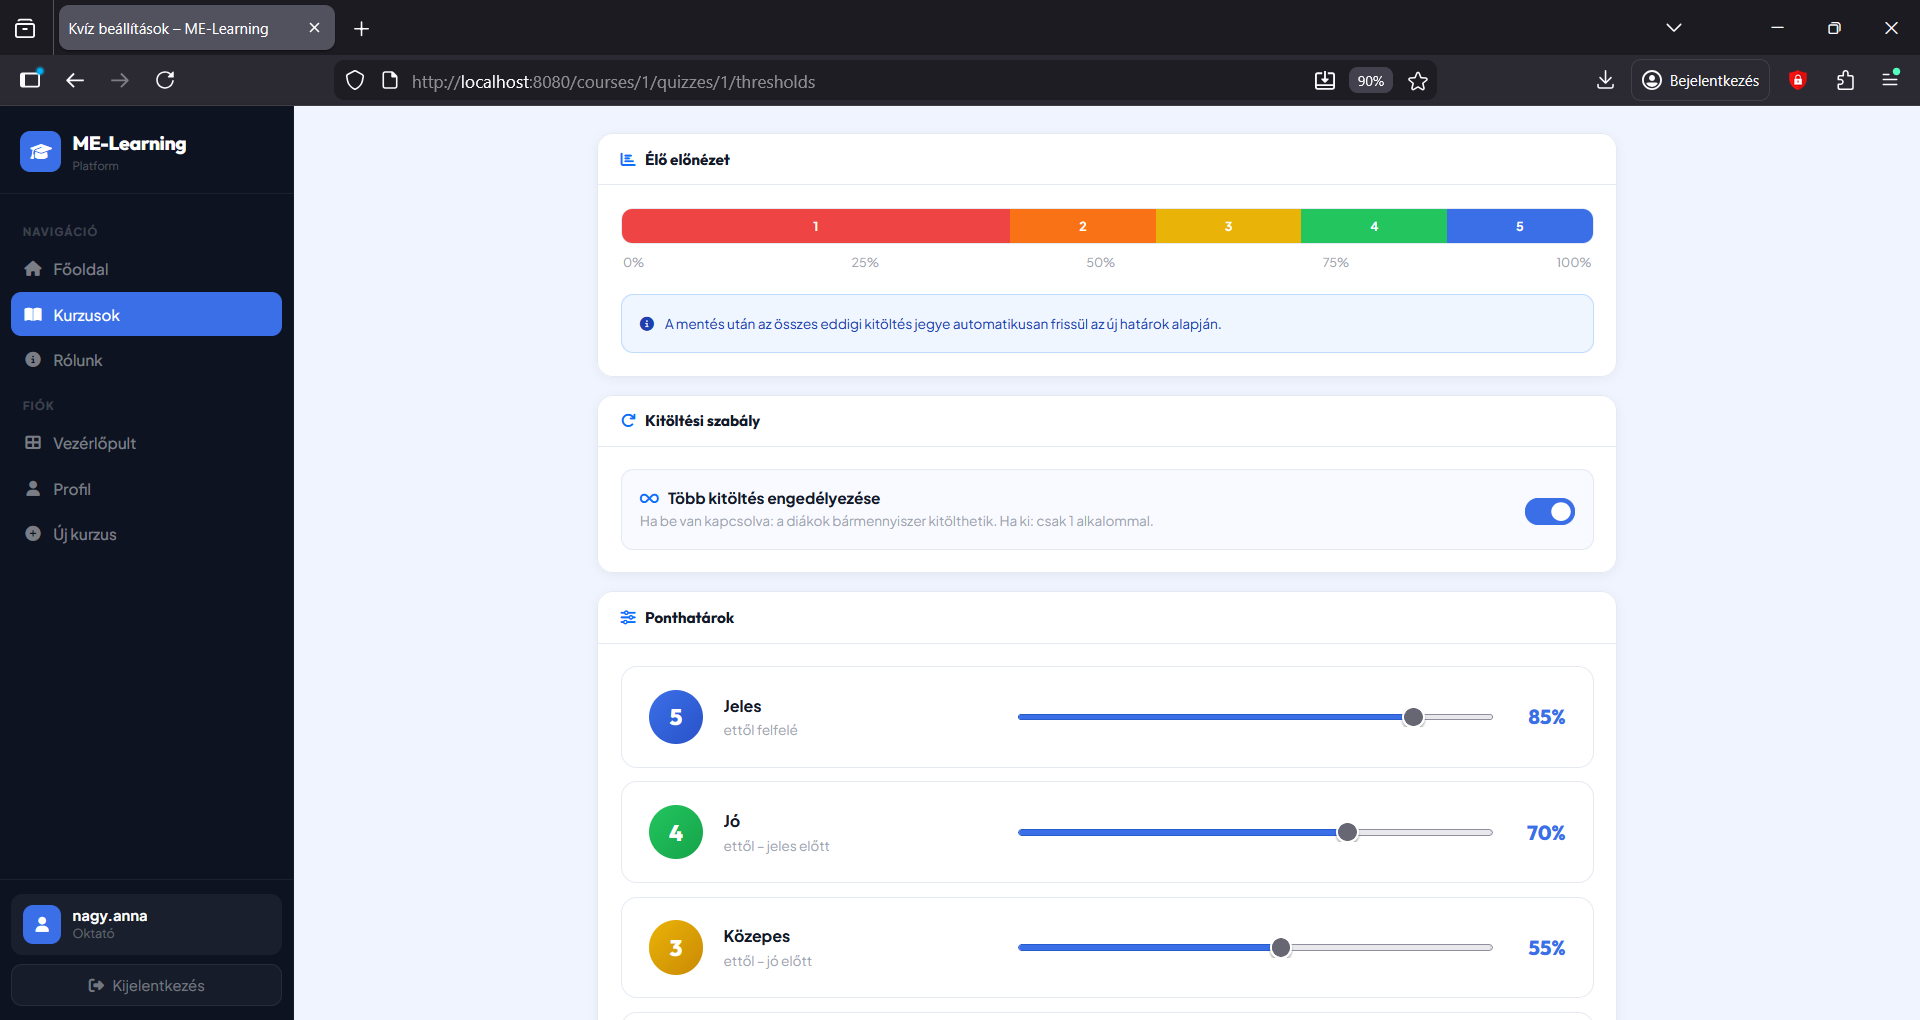
\includegraphics[width=1\textwidth]{images/Automatikus_kiertekeles.png}
    \caption{Ponthatárok beállítására szolgáló oldal}
    \label{fig:Automatikus_kiertekeles}
\end{figure}

Ez a döntés azzal az előnnyel jár, hogy az oktatók a kvíz kiértékelése után is finomíthatják a pontozási rendszert anélkül, hogy a hallgatóknak újra kellene tölteniük a tesztet.

\subsection{Eredménystatisztikák}

Az oktató az összesített eredményoldalon (\texttt{quiz-results.html}) a következő mutatókat tekintheti meg: az összes kísérlet száma, az átlagos teljesítmény százalékban, az átlagos osztályzat és az átmenési arány. Ezek a statisztikák a \texttt{QuizService}-ben kerülnek kiszámításra a tárolt \texttt{QuizResult} rekordok alapján.

\begin{figure}[h!]
    \centering
    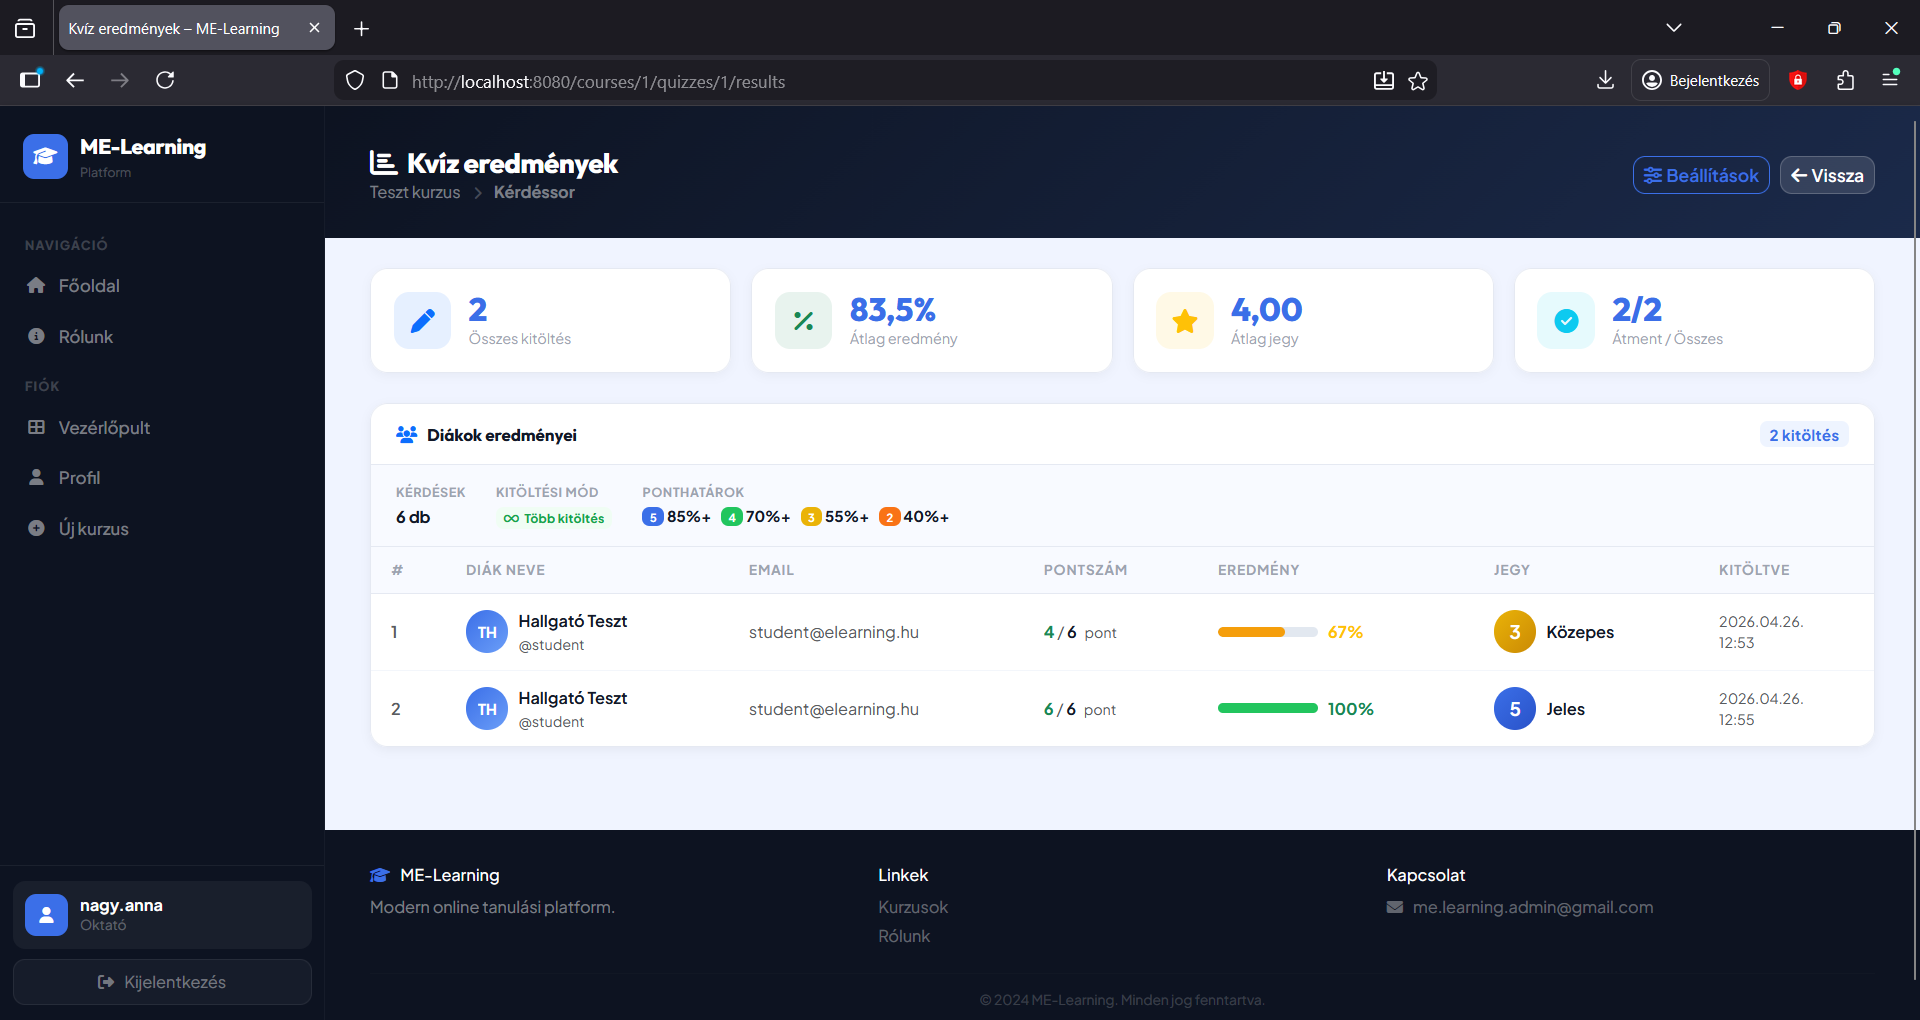
\includegraphics[width=1\textwidth]{images/Eredmenyek_megtekintese.png}
    \caption{Kvíz kitöltési eredmények megjelenítése}
    \label{fig:Eredmények_megtekintese}
\end{figure}

% ============================================================
%  3.6  Prezentáció-feldolgozás tervezése
% ============================================================
\section{Prezentáció-feldolgozás tervezése}

\subsection{Támogatott formátumok és konverziós stratégia}

Az alkalmazás PowerPoint (\texttt{.ppt}, \texttt{.pptx}) és PDF fájlok feltöltését támogatja. A tervezési cél az volt, hogy mindkét formátumot egységes módon, böngészőn belüli PDF-nézetben lehessen megjeleníteni.

PowerPoint fájlok esetén az Apache POI könyvtár segítségével minden dia \texttt{BufferedImage}-ként kerül renderelésre 3-szoros skálázási tényezővel, élesebb megjelenés érdekében. Az így kapott képek az Apache PDFBox segítségével egyetlen PDF dokumentummá fűződnek össze, amelyet az adatbázisban tárolunk. PDF fájlok esetén a konverziós lépés kihagyható: a feltöltött PDF közvetlenül tárolódik.

\subsection{Megjelenítési megközelítés}

A tárolt PDF bináris adatokat a \texttt{PresentationController} közvetlenül streameli a böngésző felé \texttt{application/pdf} MIME-típussal. A böngésző beépített PDF-megjelenítőjét alkalmazzuk, amit egy \texttt{<iframe>} elem integrál az oldalba. Ez a megközelítés nem igényel külső JavaScript könyvtárat a megjelenítéshez, és kihasználja a modern böngészők natív PDF-támogatását.

\subsection{Tárolási megfontolások}

A bináris fájladatok (\texttt{byte[]}) adatbázisban való tárolása egyszerűsíti a telepítést és az adatkonzisztenciát: nincs szükség szinkronizálásra az adatbázis és a fájlrendszer között. Ugyanakkor ez a megközelítés nagy adatmennyiség esetén növeli az adatbázis méretét. Az architektúra lazán csatolt: a \texttt{PresentationService} egy jól definiált interfészt valósít meg, amelynek implementációja a jövőben lecserélhető egy objektumtároló (pl. Amazon S3, MinIO) alapú megoldásra anélkül, hogy a kontroller vagy a nézet réteg változna.

% ============================================================
%  3.7  Réteg-struktúra a forráskódban
% ============================================================
\section{Réteg-struktúra a forráskódban}

Az alkalmazás forráskódja az alábbi csomagokba van szervezve, amelyek pontosan leképezik a háromrétegű architektúrát:

\begin{itemize}
    \item \texttt{config} – A \texttt{SecurityConfig} osztály a Spring Security szűrőlánc konfigurációját tartalmazza; a \texttt{DataInitializer} az alkalmazás első indítása során alaptesztadatokat hoz létre.
    \item \texttt{controller} – HTTP kéréseket fogadó MVC kontrollerek. Minden fő funkcionális terület saját kontrollert kap: \texttt{AuthController} (bejelentkezés, regisztráció), \texttt{CourseController} (kurzuskezelés), \texttt{DashboardController} (irányítópultok), \texttt{HomeController} (főoldal), \texttt{PresentationController} (fájl streaming), \texttt{QuizController} (kvízkezelés), \texttt{UserController} (profilkezelés, adminisztrátori felhasználókezelés).
    \item \texttt{model} – JPA entitásosztályok: \texttt{User}, \texttt{Course}, \texttt{Lesson}, \texttt{Presentation}, \texttt{Quiz}, \texttt{Question}, \texttt{QuizResult}, \texttt{Role}.
    \item \texttt{repository} – Spring Data JPA interfészek, amelyek az \texttt{JpaRepository} alaptípust terjesztik ki. Szükség esetén egyedi lekérdező metódusok (pl. \texttt{findByUsername}, \texttt{findByInstructor}) kerülnek definiálásra.
    \item \texttt{service} – Üzleti logika osztályok: \texttt{CourseService}, \texttt{QuizService}, \texttt{UserService}, \texttt{PresentationService}, \texttt{EmailService}, \texttt{CustomUserDetailsService}. A \texttt{CustomUserDetailsService} implementálja a Spring Security \texttt{UserDetailsService} interfészét.
\end{itemize}

\subsection{Függőségek iránya}

A csomagok közötti függőségek egyirányúak és hierachikusak: a \texttt{controller} csomag csak a \texttt{service} csomagtól függ, a \texttt{service} csomag a \texttt{repository} és \texttt{model} csomagoktól, a \texttt{repository} csomag csak a \texttt{model} csomagtól. Ez a struktúra megakadályozza a körkörös függőségeket, és biztosítja, hogy az egyes rétegek egymástól függetlenül módosíthatók legyenek.

% ============================================================
%  3.8  Nézetek (Thymeleaf sablonok)
% ============================================================
\section{Nézetek (Thymeleaf sablonok)}

A nézetek az alábbi könyvtárakba vannak szervezve, funkcionális területenként:

\begin{sloppypar}
\begin{itemize}
    \item \texttt{templates/} – Főoldal (\texttt{index.html}), bejelentkezés (\texttt{login.html}), regisztráció (\texttt{register.html}), profil (\texttt{profile.html}), saját kurzusok, tájékoztató oldal (\texttt{about.html}).
    \item \texttt{templates/courses/} – Kurzuslista (\texttt{list.html}), megtekintés (\texttt{view.html}), létrehozás (\texttt{create.html}), kezelés (\texttt{manage.html}), diavetítő nézet (\texttt{viewer.html}), kvízkitöltő (\texttt{take-quiz.html}), egyéni és összesített eredménynézet (\texttt{quiz-result.html}, \texttt{quiz-results.html}), ponthatár-szerkesztő (\texttt{quiz-thresholds.html}), kvíz-létrehozó (\texttt{create-quiz.html}).
    \item \texttt{templates/dashboard/} – Admin (\texttt{admin.html}), oktató (\texttt{instructor.html}) és hallgató (\texttt{student.html}) irányítópultok.
    \item \texttt{templates/presentation/} – Önálló prezentáció megjelenítő (\texttt{viewer.html}).
    \item \texttt{templates/fragments/} – Újrafelhasználható oldalsáv komponens (\texttt{sidebar.html}).
    \item \texttt{templates/error/} – 404-es hibaoldal (\texttt{404.html}) és általános hibaoldal (\texttt{error.html}).
\end{itemize}
\end{sloppypar}

A Thymeleaf sablonok természetes HTML dokumentumok, amelyek böngészőben is megnyithatók (statikus prototípusként), és csak a szerver általi feldolgozás során válnak dinamikus tartalmakká. Ez megkönnyíti a nézetek tesztelését és a frontend-fejlesztők munkáját, akiknek nem szükséges a teljes Spring Boot alkalmazást elindítaniuk a megjelenítési munkához.
